% Figura Anexo I: la curva de SAMUELSON-SOLOW (1960) como menú de política económica (en precios, EE. UU.)
\documentclass[tikz,border=3pt]{standalone}
\usepackage[T1]{fontenc}
\usepackage[utf8]{inputenc}
\usetikzlibrary{arrows.meta,calc}
\begin{document}
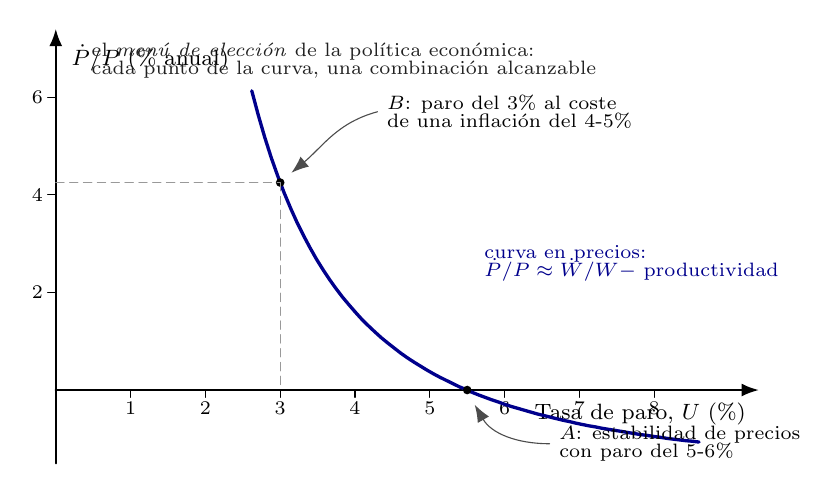
\begin{tikzpicture}[x=0.95cm, y=0.62cm, >={Latex[length=2.2mm]}, line cap=round, font=\footnotesize,
  eje/.style={->, thick},
  curva/.style={very thick},
  guia/.style={densely dashed, gray!80},
  pto/.style={circle, fill=black, inner sep=1.1pt}]
  \draw[eje] (0,-1.5) -- (0,7.4) node[below right=2pt]{$\dot{P}/P$ (\% anual)};
  \draw[eje] (0,0) -- (9.4,0) node[below left=1pt]{Tasa de paro, $U$ (\%)};
  \foreach \u in {1,2,3,4,5,6,7,8} \draw (\u,0) -- (\u,-0.15) node[below, inner sep=1.5pt]{\scriptsize\u};
  \foreach \p in {2,4,6} \draw (0,\p) -- (-0.11,\p) node[left, inner sep=1.5pt]{\scriptsize\p};
  % Curva en precios: pi = -1,8 + 54,45 U^{-2}
  \draw[curva, blue!55!black] plot[domain=2.62:8.6, samples=70] (\x,{-1.8+54.45*exp(-2*ln(\x))});
  \node[blue!55!black, align=left, anchor=west] at (5.6,2.6) {\scriptsize curva en precios:\\[-3pt]\scriptsize $\dot{P}/P \approx \dot{W}/W - $ productividad};
  % Punto A: estabilidad de precios
  \node[pto] (A) at (5.5,0) {};
  \draw[<-, gray!60!black] (5.6,-0.3) to[out=-60,in=180] (6.6,-1.1) node[right, black, align=left]{\scriptsize $A$: estabilidad de precios\\[-3pt]\scriptsize con paro del $5$-$6\%$};
  % Punto B: pleno empleo con inflación
  \node[pto] (B) at (3,4.25) {};
  \draw[guia] (3,4.25) -- (3,0);
  \draw[guia] (0,4.25) -- (3,4.25);
  \draw[<-, gray!60!black] (3.15,4.45) to[out=40,in=195] (4.3,5.7) node[right, black, align=left]{\scriptsize $B$: paro del $3\%$ al coste\\[-3pt]\scriptsize de una inflación del $4$-$5\%$};
  \node[align=left, anchor=north west, gray!25!black] at (0.35,7.3) {\scriptsize el \textit{menú de elección} de la política económica:\\[-3pt]\scriptsize cada punto de la curva, una combinación alcanzable};
\end{tikzpicture}
\end{document}
